\section{Transistorn}
\textbf{HAREC a.\ref{HAREC.a.2.6}\label{myHAREC.a.2.6}}
\label{transistorn}
\index{transistor}

\subsection{Allmänt}

\begin{wrapfigure}[12]{R}{0.5\textwidth}
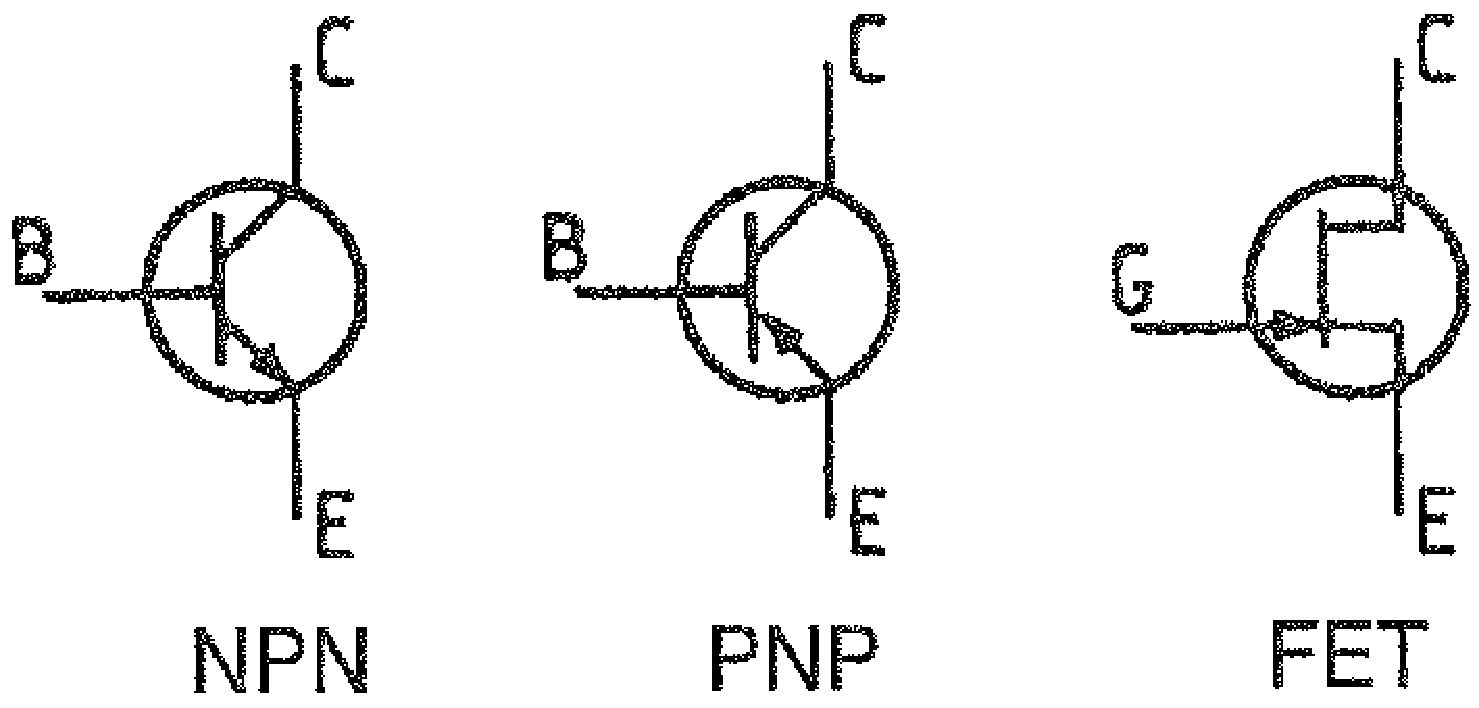
\includegraphics[width=0.5\textwidth]{images/cropped_pdfs/bild_2_2-16.pdf}
\caption{Schemasymboler}
\label{fig:BildII2-16}
\end{wrapfigure}

En transistor består av skikt av halvledarelement som sammanfogats. Vanligt är
två N-skikt och ett mellanliggande P-skikt (NPN-transistor) eller två P-skikt och
ett mellanliggande N-skikt (PNP-transistor). Skikten är försedda med
anslutningar.

Bild \ref{fig:BildII2-16}

Vanliga transistortyper
\begin{itemize}
\item NPN-transistorer (bipolära)
\item PNP-transistorer (bipolära)
\item FET-transistorer (fälteffekt-)
\end{itemize}

\subsection{NPN-transistorer}
\textbf{HAREC a.\ref{HAREC.a.2.6.1b}\label{myHAREC.a.2.6.1b}}
\index{NPN-transistor}
\index{transistor!NPN}

Halvledarskikten kallas
\begin{itemize}
\item E emitter
\item B bas
\item C kollektor
\end{itemize}

\begin{wrapfigure}{R}{0.5\textwidth}
\begin{center}
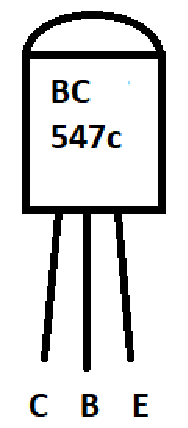
\includegraphics[width=0.1\textwidth]{images/cropped_pdfs/bild_2_6-37.pdf}
\end{center}
\caption{Transistor}
\label{fig:BildII2-17a}
\end{wrapfigure}

Bild \ref{fig:BildII2-17a}

\emph{Spärrzonerna}

\begin{wrapfigure}{R}{0.5\textwidth}
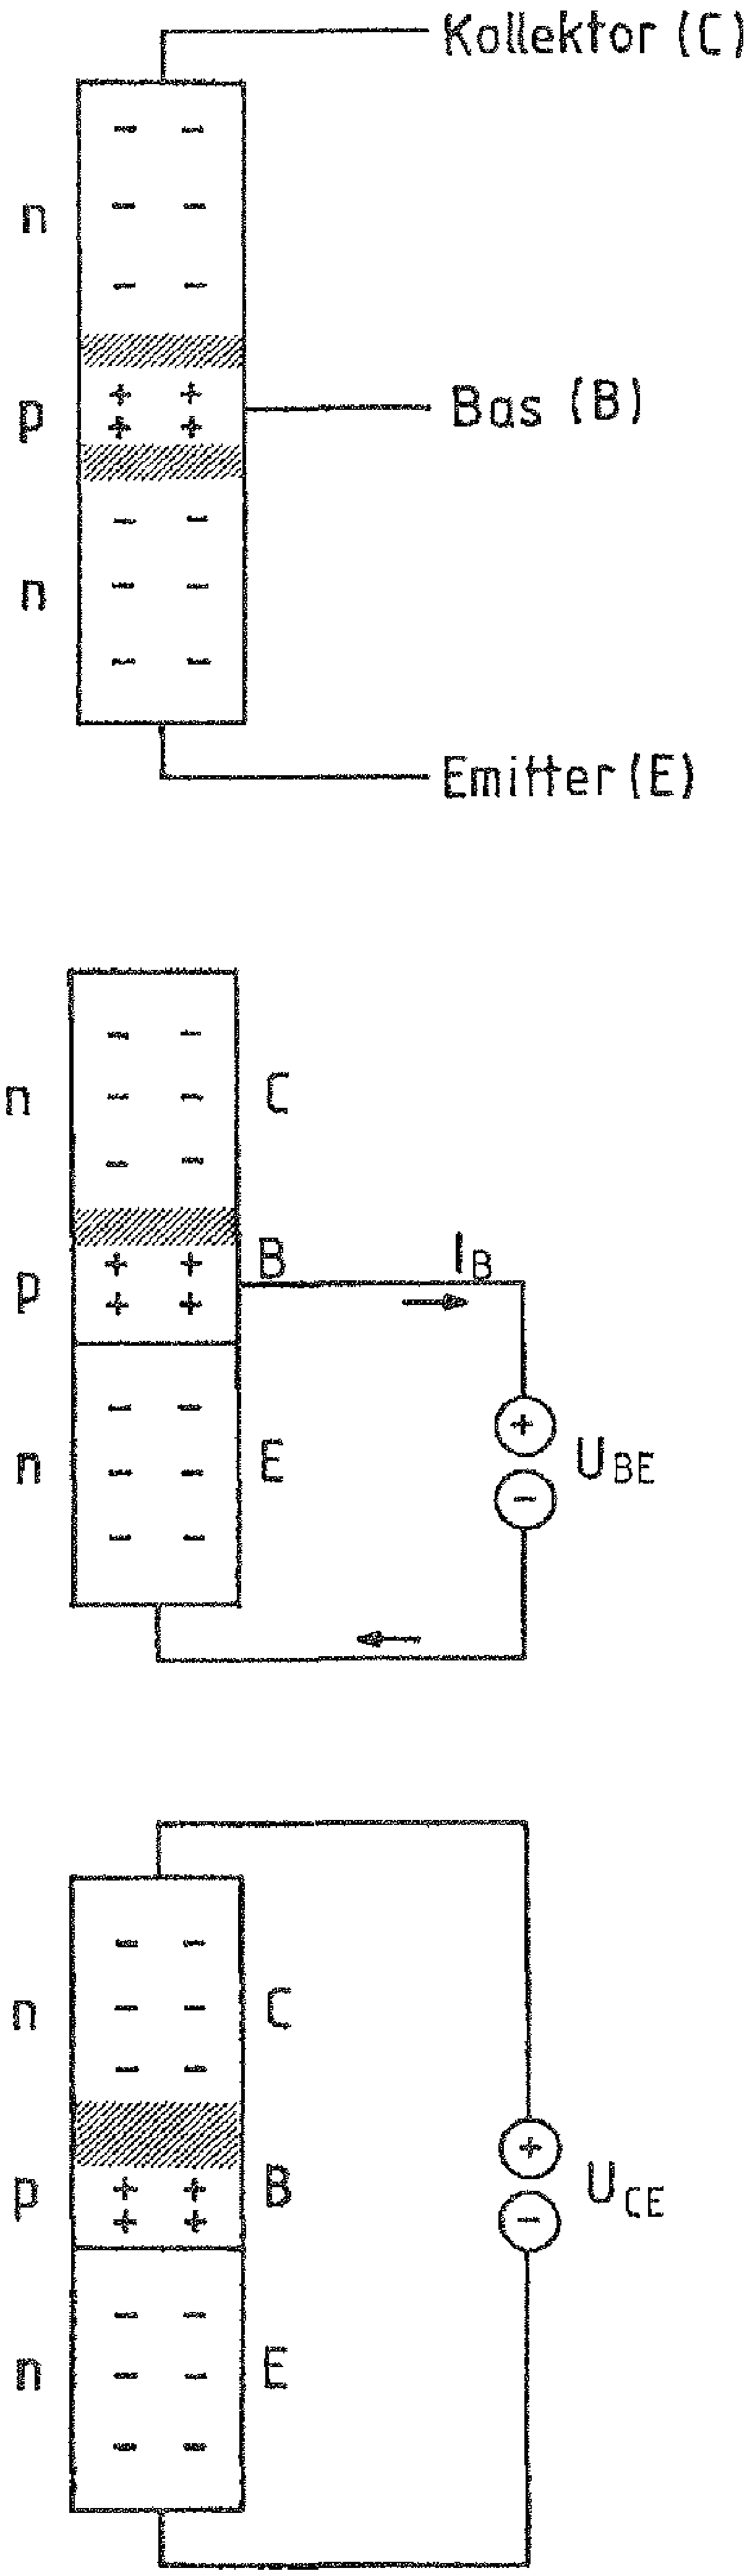
\includegraphics[width=0.5\textwidth]{images/cropped_pdfs/bild_2_2-17.pdf}
\caption{Skikten i en bipolär transistor}
\label{fig:BildII2-17}
\end{wrapfigure}

Bild \ref{fig:BildII2-17} överst

Mellan skikten B och E respektive mellan B och C bildas zoner, vars
ledningsförmåga kan styras elektriskt över anslutningarna.

Bild \ref{fig:BildII2-17} mitten

\emph{Spänningskällan \(U_{BE}\)}

Mellan bas och emitter finns en diodsträcka. När en positiv spänning läggs på
basen och en negativ spänning på emittern, så polariseras diodsträckans spärrzon
i passriktningen. Spärrzonen upplöses då och det flyter en s.k. basström
\(I_B\).

Bild \ref{fig:BildII2-17} nederst

\emph{Spänningskällan \(U_{CE}\)}

När en positiv spänning läggs på kollektorn och en negativ spänning läggs på
emittern, så polariseras diodsträckan i spärriktningen. Spärrzonen förstärks då
och det flyter ingen ström.

Bild \ref{fig:BildII2-18}

\emph{Inverkan av både \(U_{BE}\) och \(U_{CE}\)}

Två spänningskällor \(U_{BE}\) och \(U_{CE}\) ansluts till en emitterkopplad NPN-transistor.
Ur den starkt dopade emitterzonen strömmar elektronerna in i den svagt dopade
baszonen (spänning: \(U_{BE}\)). De flesta elektronerna blir emellertid inte
kvar i basen. De stöter igenom det tunna basskiktet och når fram till
kollektorskiktet med spänningen \(U_{CE}\). Det flyter en kollektorström.

För strömmen \(I_E\) (emitterström), \(I_B\) (basström) och \(I_C\)
(kollektorström) gäller:

\(I_E = I_B + I_C\) där \(I_B \ll I_C\) (\(\ll\) mycket mindre än)

Kollektorströmmen \(I_C\) kan styras med basspänningen \(U_{BE}\).

En liten ändring i basspänningen ger stor förstärkande verkan i
kollektorströmmen.

\begin{figure}
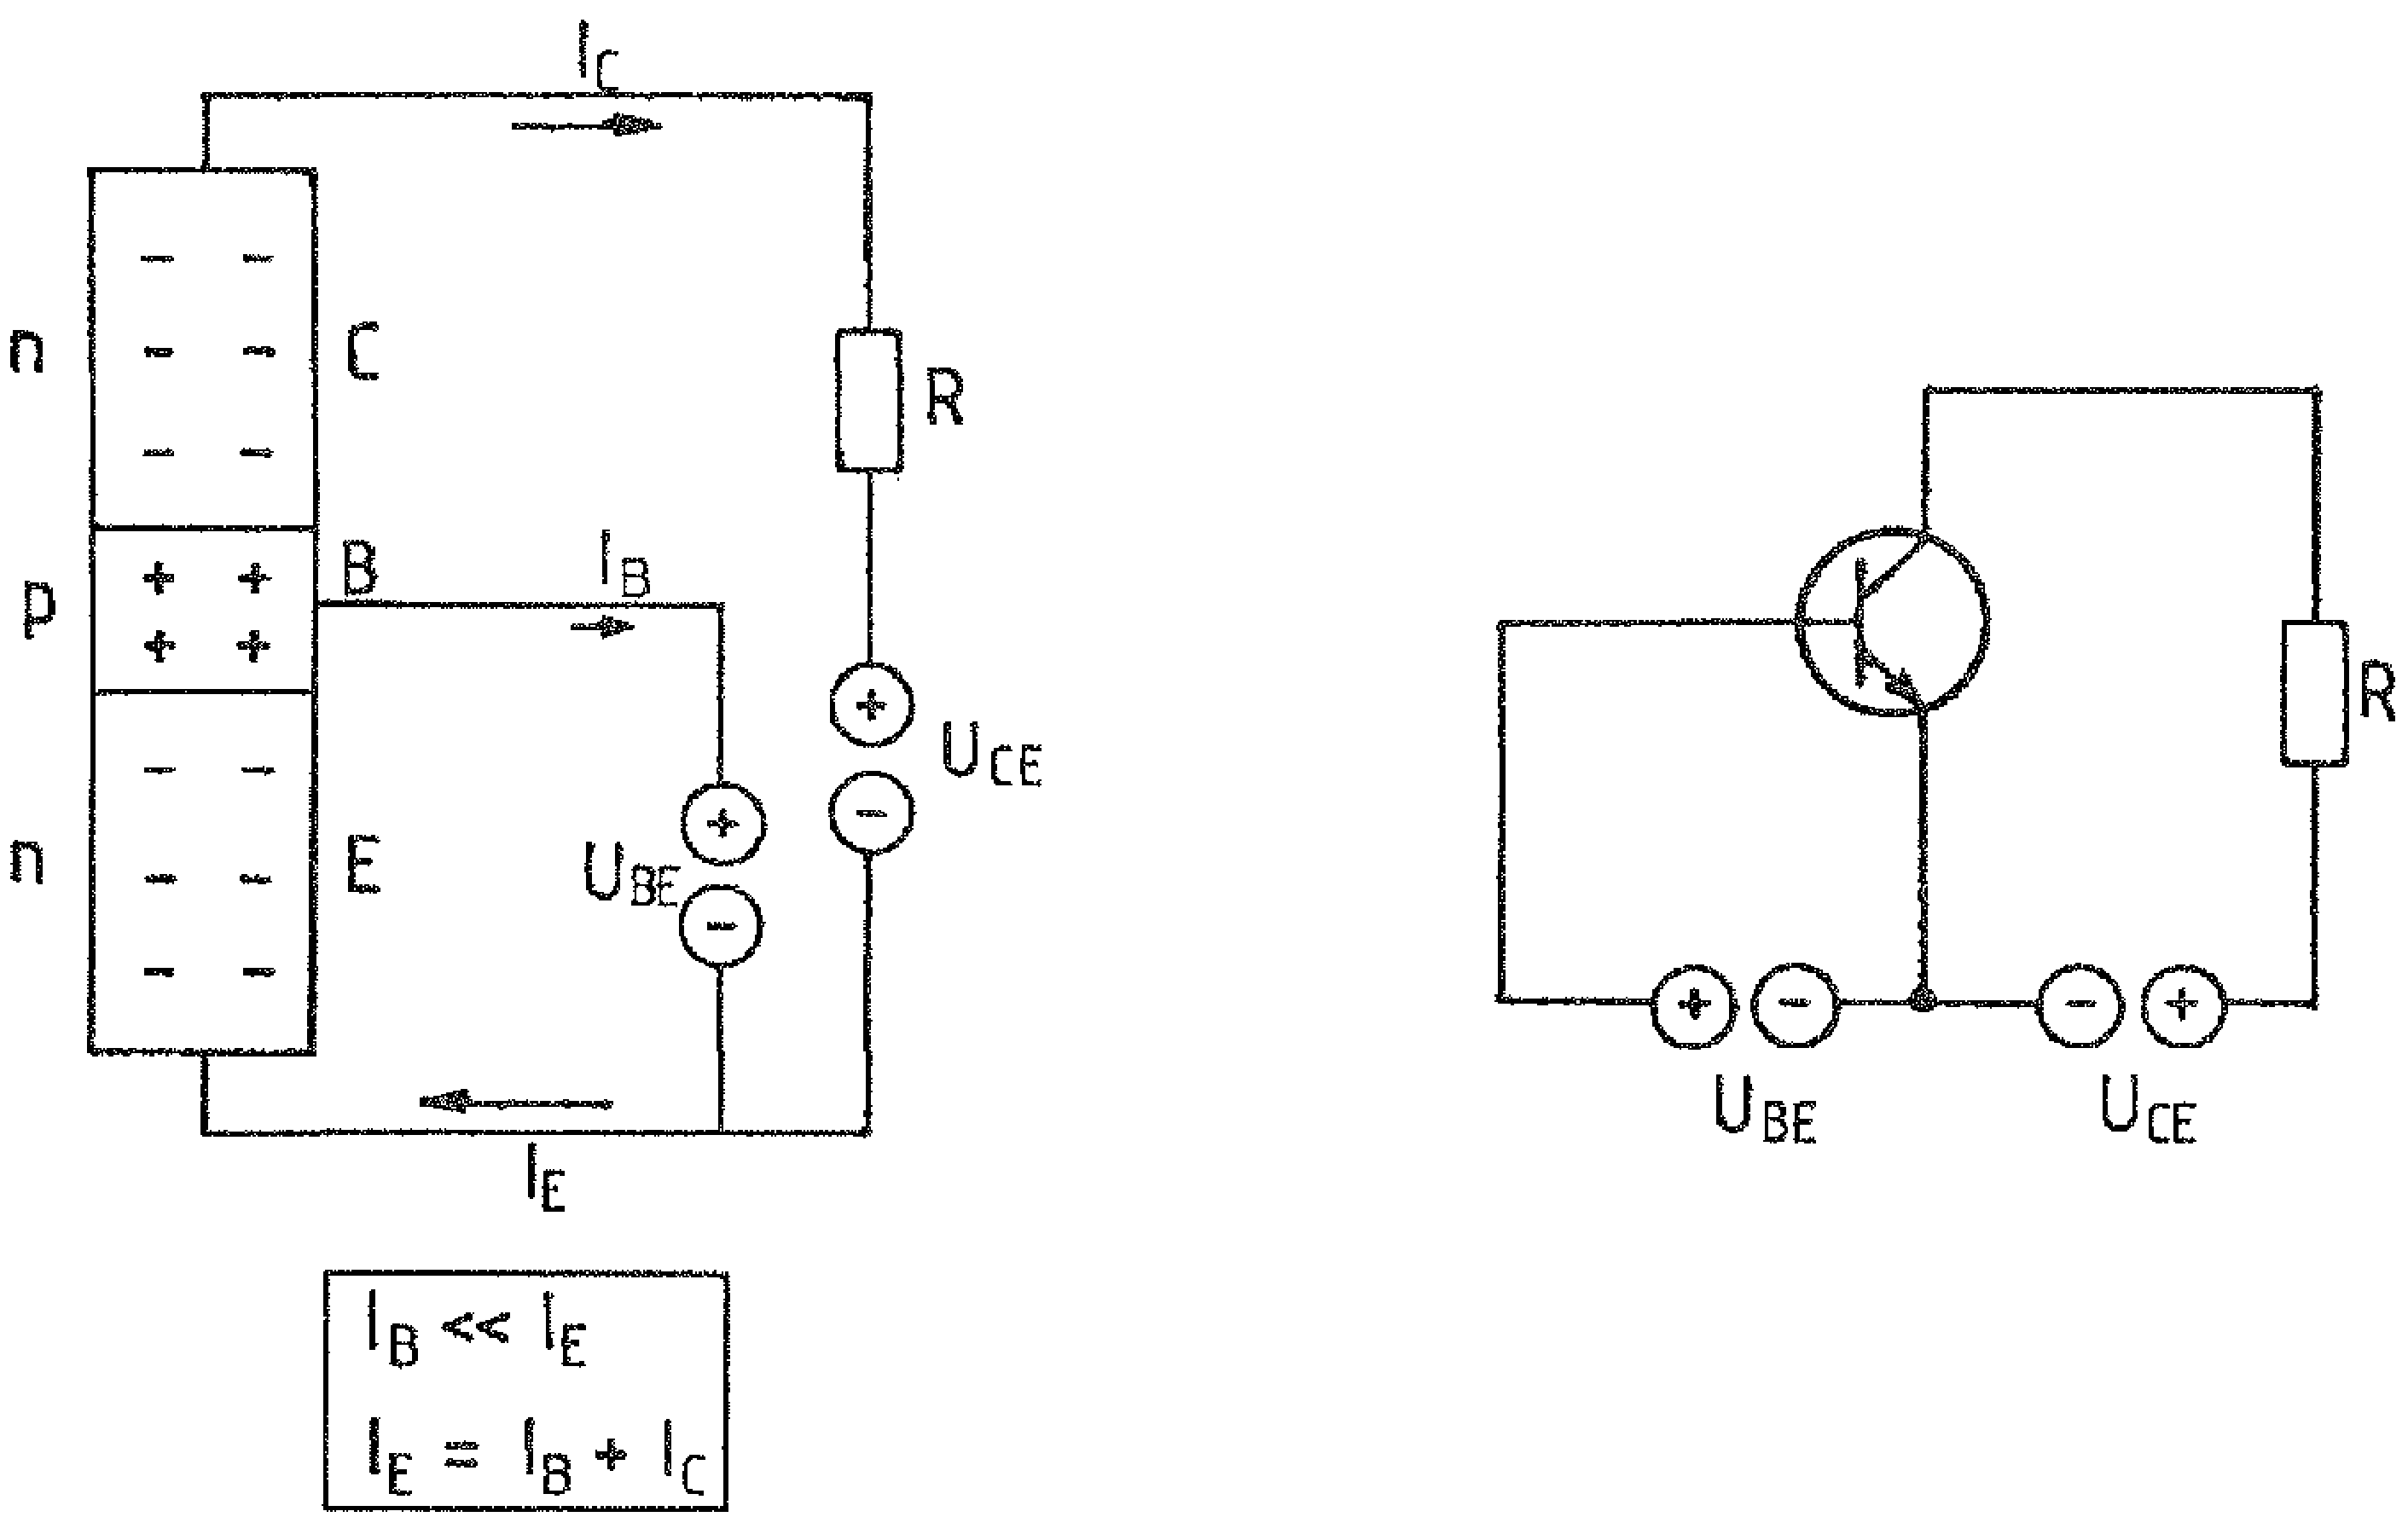
\includegraphics[width=\textwidth]{images/cropped_pdfs/bild_2_2-18.pdf}
\caption{Emitterkopplad transistor}
\label{fig:BildII2-18}
\end{figure}

\subsection{Förstärkningsfaktor}
\textbf{HAREC a.\ref{HAREC.a.2.6.2}\label{myHAREC.a.2.6.2}}
\index{förstärkningsfaktor!transistor}
\index{transistor!förstärkningsfaktor}

Om strömmen i ingångskretsen för en transistor ändras, så kan strömmen i
utgångskretsen ändras mer. Det blir då en förstärkning.

Av sambandet \(I_C = f(I_B)\) framgår strömförstärkningsfaktorn \(\beta\) eller
\(h_{FE}\) som är kvoten av ändringen i utgångsströmmen och i ingångsströmmen i
transistorns aktiva (linjära) område.

\begin{figure}
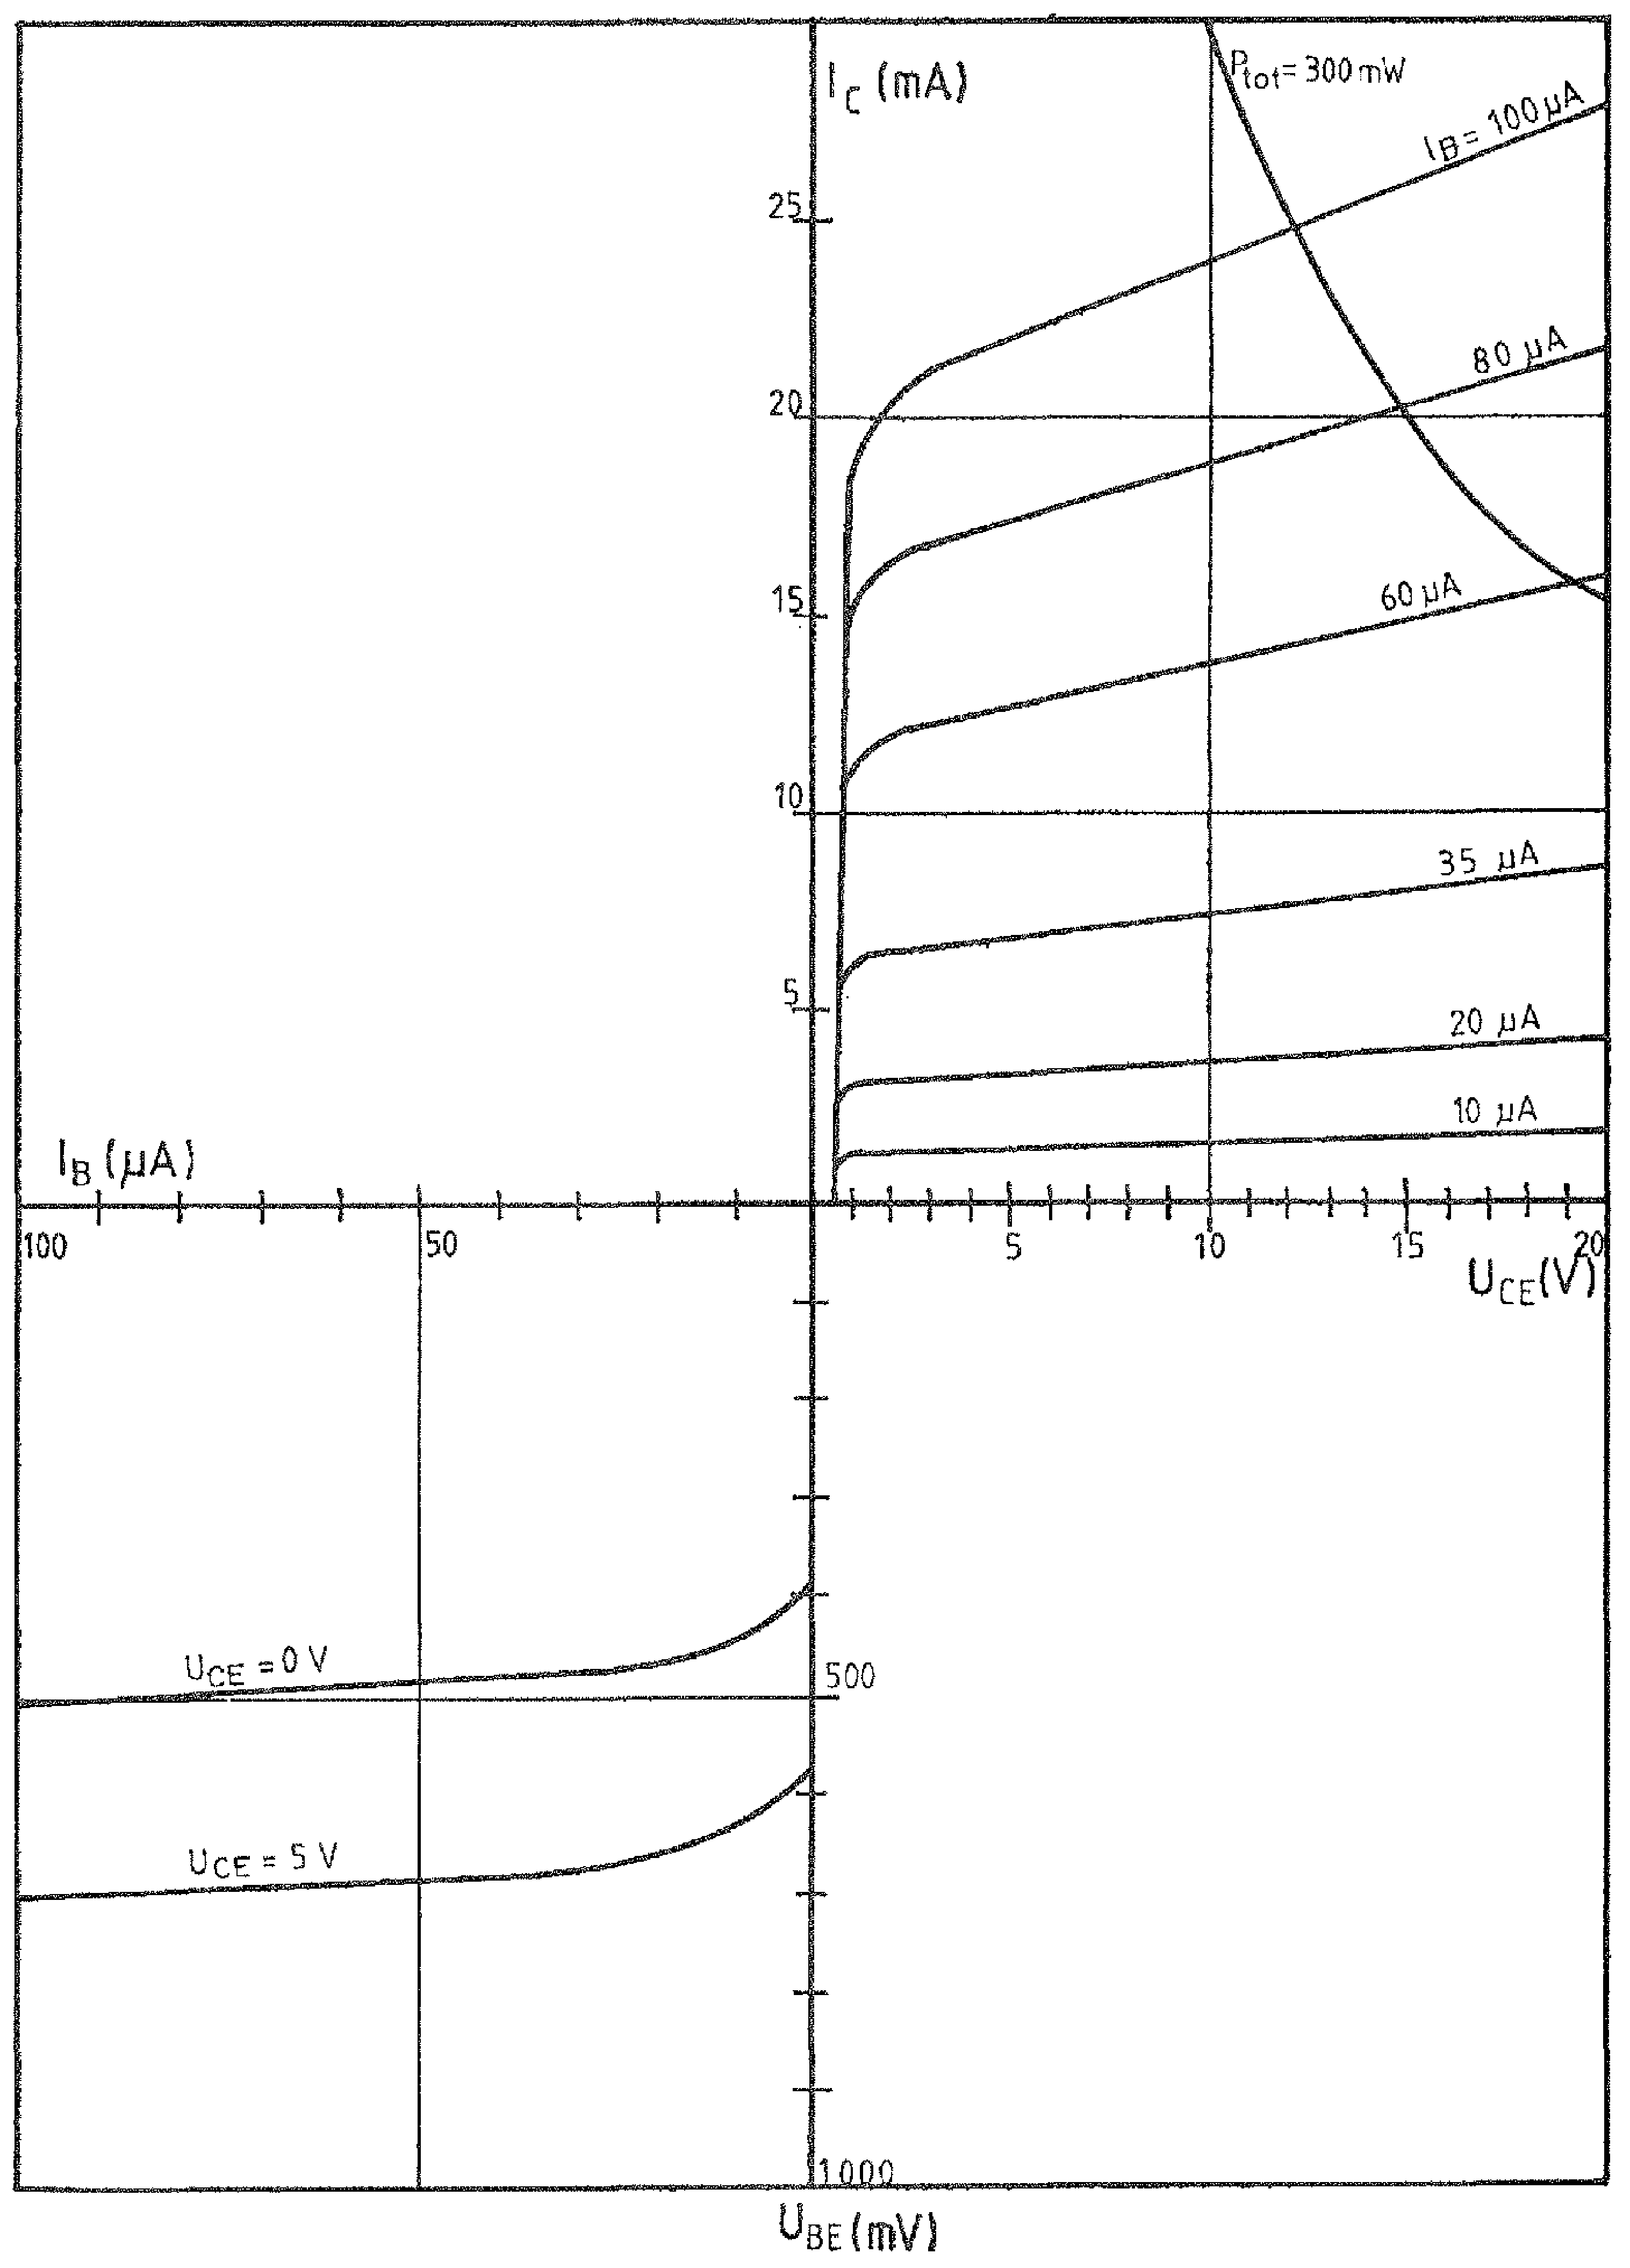
\includegraphics[width=\textwidth]{images/cropped_pdfs/bild_2_2-19.pdf}
\caption{Karaktäristika för transistor BC 107}
\label{fig:BildII2-19}
\end{figure}

Bild \ref{fig:BildII2-19}

För emitterkoppling gäller:

\(h_{FE} = \dfrac{\Delta I_C}{\Delta I_B}\)

\begin{tabular}{ll}
  \(h_{FE}\) & strömförstärkningsfaktorn \\
  \(\Delta I_c\)   & ändringen i kollektorströmmen \\
  \(\Delta I_B\)   & ändringen i basströmmen \\
\end{tabular}

\subsection{PNP-transistorer}
\textbf{HAREC a.\ref{HAREC.a.2.6.1a}\label{myHAREC.a.2.6.1a}}
\index{PNP-transistor}
\index{transistor!PNP}

Ersätter man de två N-skikten i en NPN-transistor med P-skikt och P-skiktet med
ett N-skikt så erhåller man en PNP-transistor.

Uppbyggnad, koppling och användning av en PNP-transistor motsvarar i övrigt den
för en NPN-transistor. Spänningskällorna måste emellertid ha motsatt polaritet.

\subsection{Fälteffekttransistorer}
\textbf{HAREC a.\ref{HAREC.a.2.6.3}\label{myHAREC.a.2.6.3}}
\index{fälteffekttransistor}
\index{transistor!fälteffekt}
\index{FET}
\index{transistor!FET}

\emph{Allmänt}

Fälteffekttransistorer (förkortat FET) har mycket hög ingångsimpedans och
styrströmmen blir därför mycket svag. Man säger därför att en FET är
spänningsstyrd.

Även NPN- och PNP-transistorer -- kallade bipolära transistorer -- styrs med
spänning, men dessa typer har en relativt lågt ingångsimpedans och därför högre
styrström. Man säger därför att de är strömstyrda.

\begin{wrapfigure}[6]{R}{0.5\textwidth}
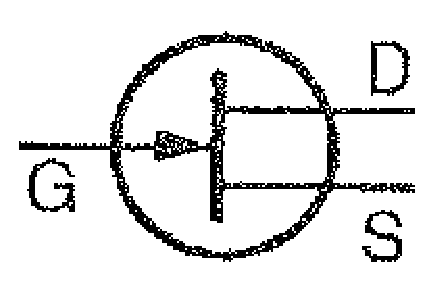
\includegraphics[width=0.5\textwidth]{images/cropped_pdfs/bild_2_2-20.pdf}
\caption{Schemasymbol för en FET}
\label{fig:BildII2-20}
\end{wrapfigure}

Bild \ref{fig:BildII2-20}

Fälteffekttransistorn har tre anslutningar (elektroder):

\begin{tabular}{ll}
  S & source (katod) \\
  D & drain (anod) \\
  G & gate (grind, styre) \\
\end{tabular}

\begin{wrapfigure}{R}{0.5\textwidth}
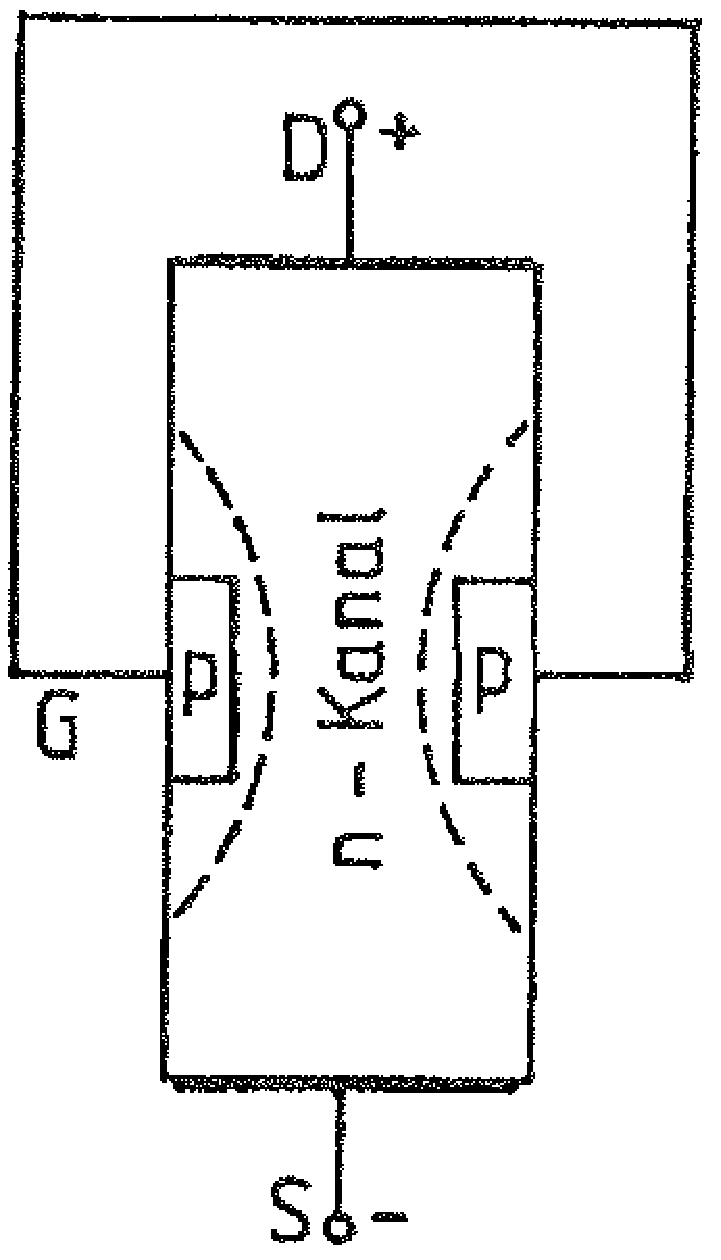
\includegraphics[width=0.5\textwidth]{images/cropped_pdfs/bild_2_2-21.pdf}
\caption{Skikten i en N-kanal FET}
\label{fig:BildII2-21}
\end{wrapfigure}

\emph{Fälteffekttransistorns uppbyggnad}

Bild \ref{fig:BildII2-21}

Bilden visar ett N-ledande skikt (även kallat N-kanal) med elektroderna S och D
anslutna till respektive ändar av skiktet. N-kanalen passerar mellan två
P-ledande skikt förbundna med styrelektroden G.

När en spärrspänning läggs mellan G och S, så breder spärrskikten ut sig och
N-kanalen blir trängre. Läggs en negativ spänning på S och en positiv spänning
på D, så kommer det att flyta en ström i N-kanalen. Strömmens styrka kan
påverkas med spänningen på G.

En liten spänningsändring \(\Delta U_{GS}\) medför stor ändring av strömmen
\(\Delta I_{GS}\) i N-kanalen. Detta innebär förstärkning.

\begin{wrapfigure}{R}{0.5\textwidth}
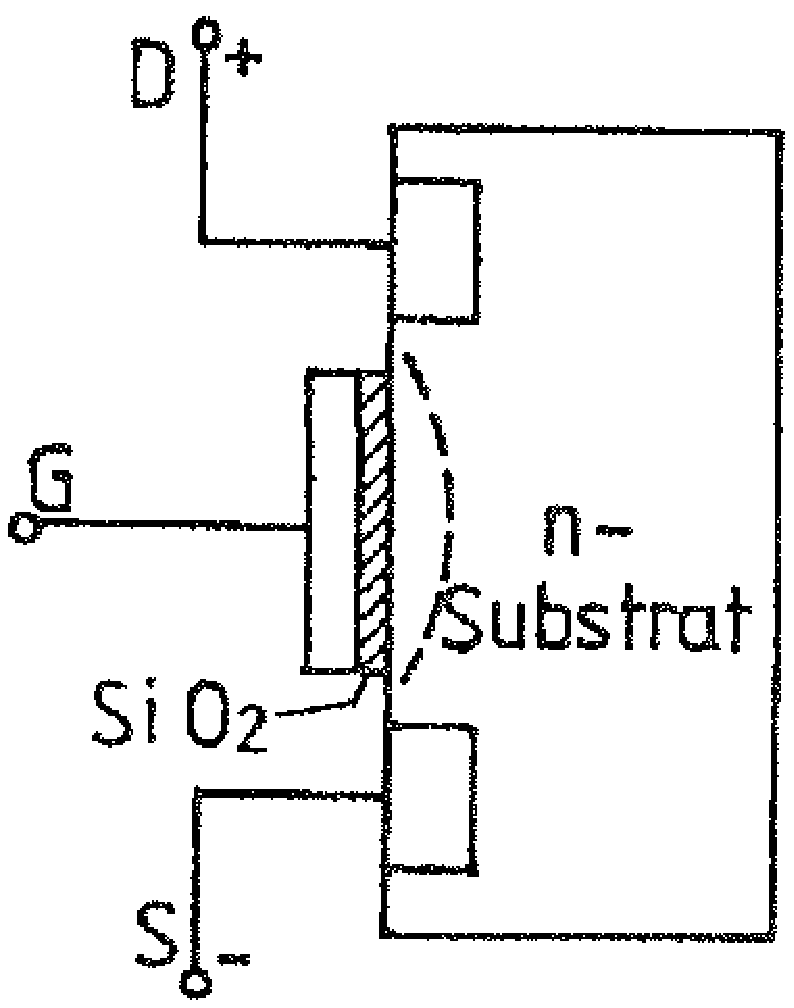
\includegraphics[width=0.5\textwidth]{images/cropped_pdfs/bild_2_2-22.pdf}
\caption{Skikten i en N-kanal MOSFET}
\label{fig:BildII2-22}
\end{wrapfigure}


Bild \ref{fig:BildII2-22}

\index{MOSFET}
\index{transitor!MOSFET}

I en Metal Oxide Semicoductor Field Effect Transistor (MOSFET) är
G-elektroden isolerad med ett kiseloxidskikt, trots att namnet förespeglar
ett metalloxidskikt. Funktionssättet är samma som för en FET.
Drain-strömmen kan ökas eller minskas med hjälp av en
positiv respektive negativ spänning på G.
%\url{https://en.wikipedia.org/wiki/MOSFET}

\emph{Resistansen mellan gate och source}

För att erhålla en förstärkning med en FET, sätter man in en resistor
\(R_0\) i drain-strömkretsen. Över resistorn uppstår då spänningsändringar i
proportion med strömändringarna.

För att fastställa viloströmmen och därmed arbetspunkten för samma transistor
sätter man in en resistor \(R_S\) i source-strömkretsen. storleken på
source-resistorn ger sig av önskad gate-förspänning \(-U_{GS}\).

\(R_S = \dfrac{-U_{GS}}{I_D}\)

\subsection{Sambandet drain-ström och spänning}

\begin{wrapfigure}{R}{0.5\textwidth}
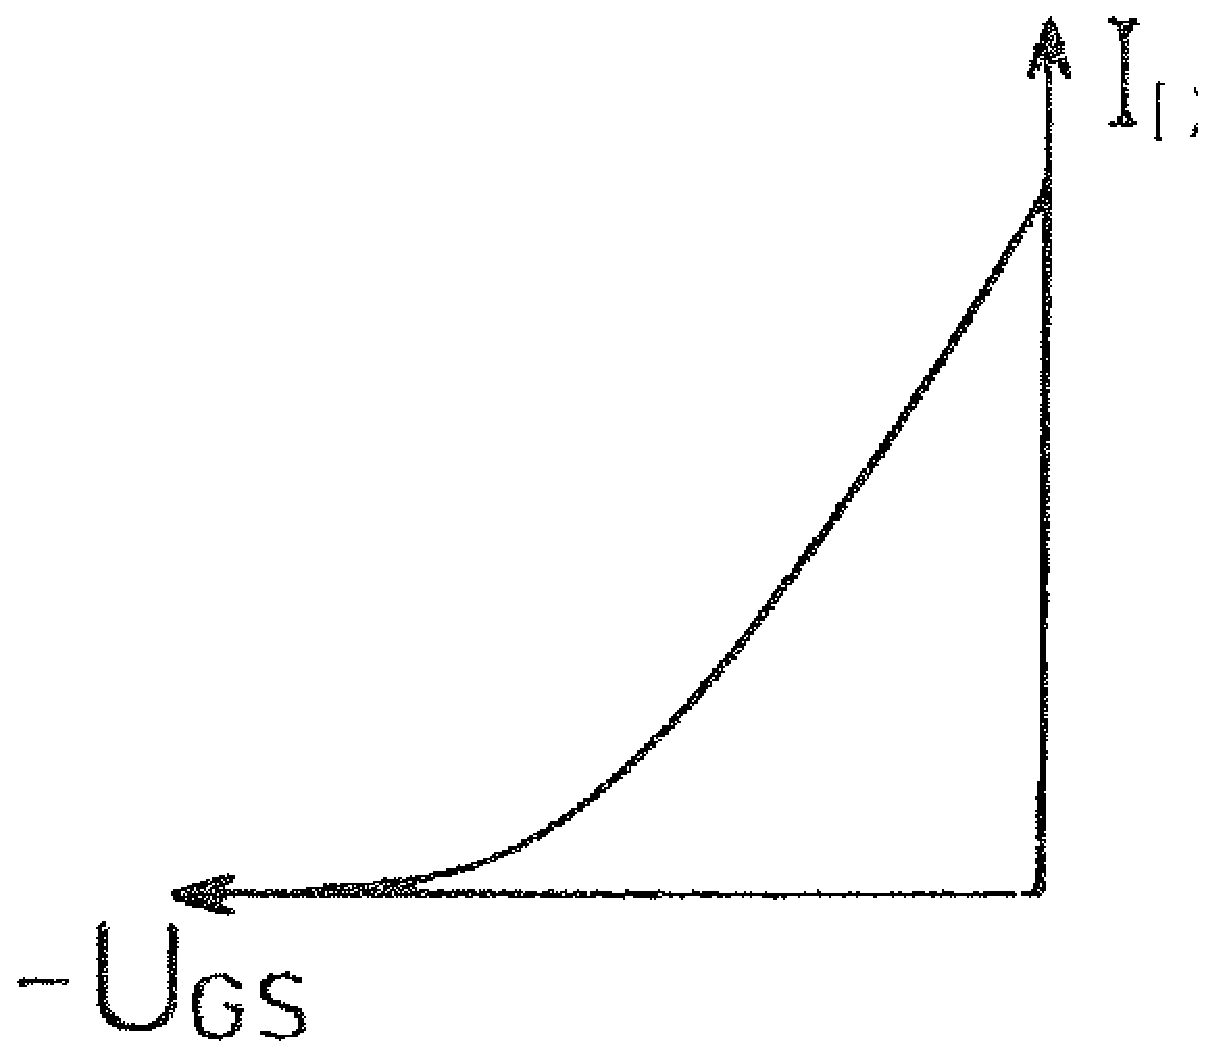
\includegraphics[width=0.5\textwidth]{images/cropped_pdfs/bild_2_2-23.pdf}
\caption{Karaktäristik för N-kanal FET}
\label{fig:BildII2-23}
\end{wrapfigure}

Bild \ref{fig:BildII2-23}

För att beskriva en FET använder man sig av karaktäristiska kurvor. Vi har redan
presenterat bipolära transistorers in- och utgångsegenskaper i kurvform.
Eftersom ingångsströmmen (gateströmmen) i en FET är praktiskt taget noll, så är
en sådan kurva utan praktisk mening. I stället framställer man grafiskt
sammanhanget mellan styrspänningen \(U_{GS}\) och utgångsströmmen (drainströmmen
\(I_D\)). Eftersom det finns N-kanal FET och P-kanal FET så skiljer polariteten
på \(U_{GS}\) för dessa båda typer.
